\documentclass{paper}

\title{Kryptographie \\ Rivest-Shamir-Adleman-Kryptosystem}
\author{Niklas Simandi}
\date{18. März 2022}

\pgfplotsset{compat=1.18,width=10cm}

\newtheoremstyle{classic}{ }{0mm}{}{0mm}{\bfseries}{:}{ }{}
\theoremstyle{classic}
\newtheorem{definition}{Definition}[section]
\newtheorem{remark}[definition]{Bemerkung}
\newtheorem{theorem}[definition]{Satz}

\pagenumbering{gobble}

\begin{document}

\maketitle

\begin{abstract}\sloppy\noindent
Nach einer Einführung in Public-Key-Kryptosysteme ist das Rivest-Shamir-Adleman-Kryptosystem exemplarisch hinsichtlich der Chiffrierung, der Dechiffrierung und dem Schlüsselaustausch dargelegt.
\end{abstract}

\tableofcontents

\newpage

\pagenumbering{arabic}

\section{Kryptographie}

Kryptographie ist die Lehre von Geheimschriften zur Wahrung vertraulicher Informationen vor Unbefugten. Das Ausgangsproblem der Kryptographie ist die Kommunikation über einen von Natur aus unsicheren Kanal. Die zu versendende Information heißt \textbf{Klartext}. Durch den Prozess der \textbf{Chiffrierung} erzeugt der Sender aus einem Klartext einen \textbf{Geheimtext}, der im Idealfall nur für den Empfänger reversibel ist. Für die Chiffrierung und Dechiffrierung ist jeweils ein \textbf{Schlüssel} nötig. Die nachfolgende Definition präzisiert die Beziehung zwischen diesen Begriffen.
\begin{definition}
\label{def:1.1}
Sei \(\mathcal{P}\) eine Menge von Klartexten, \(\mathcal{C}\) eine Menge von Geheimtexten und \(\mathcal{K}\) eine Menge von Schlüsseln. Ein \textbf{Kryptosystem} \((\mathcal{P},\mathcal{C},\mathcal{K})\) definiert für alle \(k \in \mathcal{K}\) eine \textbf{Chiffrierungsregel} \(e_k : \mathcal{P} \rightarrow \mathcal{C}\) und eine zugehörige \textbf{Dechiffrierungsregel} \(d_j : \mathcal{C} \rightarrow \mathcal{P}\) für ein \(j \in \mathcal{K}\), sodass \(d_j(e_k(p)) = p\) für alle \(p \in \mathcal{P}\) gilt.
\end{definition}
Der Kommunikationsablauf ist nun im Allgemeinen wie folgt:
\begin{enumerate}
\item Zu Beginn einigen sich Sender und Empfänger auf ein Kryptosystem \((\mathcal{P},\mathcal{C},\mathcal{K})\) und ein \textbf{Schlüsselpaar} \((k,j) \in \mathcal{K} \times \mathcal{K}\) mit \(d_j(e_k(p)) = p\) für alle \(p \in \mathcal{P}\).
\item Der Sender sendet den Geheimtext \(c \coloneqq e_k(p)\) für den Klartext \(p \in \mathcal{P}\) über einen Kanal an den Empfänger.
\item Der Empfänger dechiffriert den empfangenen Geheimtext \(c\), um den Klartext \(p\) aus \(d_j(c)\) zu erhalten.
\end{enumerate}
Zu beachten ist allerdings, dass dieser Ablauf eine Einigung zwischen Sender und Empfänger auf das Schlüsselpaar \((k,j)\) voraussetzt. Dies ist in der Realität nur selten der Fall. In der Regel geschieht der \textbf{Schlüsselaustausch} stattdessen über den Kommunikationskanal selbst.

Vorweg ist dies zum Beispiel beim Rivest-Shamir-Adleman-Kryptosystem gegeben, dessen Schlüsselaustausch auf dem Diffie-Hellman-Protokoll basiert \cite{pkx:1976}, das \(k\) als den \textbf{öffentlichen Schlüssel} und \(j\) als den \textbf{privaten Schlüssel} bezeichnet \cite{rsa:1977}.

Ziel der Facharbeit ist das Zusammenspiel zwischen öffentlichem und privatem Schlüssel konkret für das Rivest-Shamir-Adleman-Kryptosystem darzustellen. Das heißt, die Chiffrierungsregel und Dechiffrierungsregel zu bestimmen.

\subsection{Codierungen}

Der Austausch von Informationen, auch Kommunikation, basiert auf vordefinierten Regeln und Vereinbarungen. In der Kryptographie dient ein \textbf{Code} als System zur Kommunikation zwischen Sender und Empfänger. Besonders für Kryptosysteme ist die Etablierung eines Codes zur numerischen Betrachtung von Nachrichten unabdingbar.
\begin{definition}
\label{def:1.2}
Sei \(n \in \N\). Eine Menge \(\Sigma \coloneqq \{a_1,\dots,a_n\}\) heißt \textbf{Alphabet}, falls jedes \textbf{Zeichen} \(a_i\) mit \(1 \leq i \leq n\) einzigartig in \(\Sigma\) ist. Eine Zeichenfolge \(\textbf{w} \coloneqq w_1 w_2 \dots w_l\) mit \(l \in \N\) heißt \textbf{Wort}, wobei \(w_j \in \Sigma\) für alle \(1 \leq j \leq l\) ist.
\end{definition}
Sei fortan \(\mathbb{L} \coloneqq \{\texttt{A},\texttt{B},\dots,\texttt{Z}\}\) das Alphabet der 26 lateinischen Großbuchstaben. Eine Nachricht ist so durch Anpassen von Umlauten, Großbuchstaben, Wortzwischenräumen und Satzzeichen in ein Wort aus \(\mathbb{L}\) überführbar und umgekehrt. Des Weiteren ist die Äquivalenz von Alphabeten ausschließlich von der Anzahl der Zeichen abhängig, wie die nachfolgende Definition verdeutlicht.
\begin{definition}
\label{def:1.3}
Sei \(n \in \N\), und seien \(\Sigma_A \coloneqq \{a_1,\dots,a_n\},\Sigma_B \coloneqq \{b_1,\dots,b_n\}\) Alphabete. Eine Funktion der Form \(\phi : \Sigma_A \rightarrow \Sigma_B, a_i \mapsto b_i\) mit \(1 \leq i \leq n\) heißt \textbf{Codierung} über \(\Sigma_A\) und \(\Sigma_B\). Ferner ist ein Wort \(\textbf{x} \coloneqq x_1 x_2 \dots x_m\) mit \(x_i \in \Sigma_A\) genau dann äquivalent zu \(\textbf{y} \coloneqq y_1 y_2 \dots y_m\) mit \(y_i \in \Sigma_B\), falls \(\phi(x_i) = y_i\) für alle \(1 \leq i \leq m\) gilt.
\end{definition}
Sei \(\Z_n \coloneqq \{0,\dots,n - 1\}\) mit \(n \in \N\) und \(n > 1\) ein Alphabet in \(n\) Zeichen. Dann ist durch nachfolgende Tabelle eine Codierung \(\psi\) über den Alphabeten \(\mathbb{L}\) und \(\Z_{26}\) gegeben.
\begin{table}[ht]\renewcommand{\arraystretch}{\baselinestretch}\centering
\caption{Jeder Buchstabe entspricht der darunter stehenden Zahl}
\vspace{6pt}
{\ttfamily
\begin{tabular}{r r r r r r r r r r r r r}
A & B & C & D & E & F & G & H & I & J & K & L & M \\
0 & 1 & 2 & 3 & 4 & 5 & 6 & 7 & 8 & 9 & 10 & 11 & 12 \\
N & O & P & Q & R & S & T & U & V & W & X & Y & Z \\
13 & 14 & 15 & 16 & 17 & 18 & 19 & 20 & 21 & 22 & 23 & 24 & 25
\end{tabular}
}
\label{tab:1}
\end{table}

Diese willkürlich gewählte Codierung erlaubt nun die numerische Betrachtung beliebiger Nachrichten. Nach Anpassen unzulässiger Zeichen entspricht eine Nachricht wie zum Beispiel "`Seebär"' dem Wort \(\textbf{x} \coloneqq \texttt{S\;E\;E\;B\;A\;E\;R}\). Insbesondere ist \textbf{x} bezüglich \(\psi\) äquivalent zu \(\textbf{y} \coloneqq \texttt{18\;4\;4\;1\;0\;4\;17}\).

\subsection{Public-Key-Kryptosystem}

Nach der Festlegung eines Codes folgt nun eine Präzisierung von Definition \ref{def:1.1} auf bestimmte Kryptosysteme, wo der Schlüsselaustausch über den unsicheren Kommunikationskanal stattfindet.
\begin{definition}
\label{def:1.4}
Ein \textbf{Public-Key-Kryptosystem} \((\mathcal{P},\mathcal{C},\mathcal{K})\) bestimmt einen privaten Schlüssel \(j \in \mathcal{K}\) zur Dechiffrierung und einen zugehörigen öffentlichen Schlüssel \(k \in \mathcal{K}\) zur Chiffrierung. Die Dechiffrierungsregel \(d_j : \mathcal{C} \rightarrow \mathcal{P}\) sei invers zur Chiffrierungsregel \(e_k : \mathcal{P} \rightarrow \mathcal{C}\) mit \(d_j(e_k(p)) = p\) für alle \(p \in \mathcal{P}\) und \(e_k(d_j(c)) = c\) für alle \(c \in \mathcal{C}\). Insbesondere sei die Berechnung der inversen Funktion von \(e_j\) nur dann durchführbar, falls zusätzlich der private Schlüssel bekannt ist \cite{pkx:1976}.
\end{definition}
Eine Funktion mit der beschriebenen Eigenschaft heißt \textbf{Falltürfunktion}. Ferner ist die Zusatzinformation dann die \textbf{Falltür}. Basierend auf der Annahme, dass Falltürfunktionen existieren, ist der Schlüsselaustausch nun über einen unsicheren Kommunikationskanal realisierbar.
\begin{remark}
\label{rem:1.5}
Zu Beginn einigen sich Sender und Empfänger auf einen Code zur Nutzung in einem Public-Key-Kryptosystem \((\mathcal{P},\mathcal{C},\mathcal{K})\). Sei \(m \in \mathcal{P}\) die codierte Nachricht, die an den Empfänger zu senden ist.
\begin{enumerate}
\item Der Empfänger bestimmt einen privaten Schlüssel \(j \in \mathcal{K}\) und einen öffentlichen Schlüssel \(k \in \mathcal{K}\) mit \(d_j(e_k(p)) = p\) für alle \(p \in \mathcal{P}\).
\item Der Sender bestimmt die Chiffrierungsregel \(e_k\) durch den öffentlichen Schlüssel \(k\). Nun ist der Sender in der Lage, Klartexte zu chiffrieren und so den Geheimtext \(c \coloneqq e_k(m)\) zu versenden.
\item Der Empfänger dechiffriert den empfangen Geheimtext \(c\) gemäß \(d_j(c)\), um wiederum \(m\) zu erhalten.
\end{enumerate}
\end{remark}
Da lediglich der Empfänger \(d_j\) kennt, ist in der Theorie die Kommunikation zwischen Sender und Empfänger abhörsicher. Allerdings bleibt fraglich, ob Falltürfunktionen wie in Definition \ref{def:1.4} beschrieben in der Praxis existieren. Die moderne Kryptographie weitet deswegen den Begriff einer Falltürfunktion auch auf Funktionen aus, deren inverse Funktion nur mit einem hohen Rechenaufwand ohne Zusatzinformation zu bestimmen ist, da ein Unbefugter nur über begrenzte Ressourcen und Rechenleistung verfügt, ist diese Neudefinition sinnvoll.

\section{Elementare Zahlentheorie}

Das Rivest-Shamir-Adleman-Kryptosystem beruht auf etwaigen Überlegungen der elementaren Zahlentheorie, also der Studie der Phänomene ganzer Zahlen. Sei fortan \(\mathbb{P}\) die Menge aller Primzahlen.

\subsection{Faktorisierungsproblem}

Grundlage für die Falltür des Rivest-Shamir-Adleman-Kryptosystems bildet das Faktorisierungsproblem, das auf klassischen Computern vermutlich nur schwer zu lösen ist \cite{ifa:2020}.
\begin{theorem}
\label{thm:2.1}
Sei \(n \in \N\) mit \(n > 1\). Dann gibt es eindeutig bestimmte Primzahlen \(p_1,\dots,p_m \in \mathbb{P}\) mit \(p_1 < \dots < p_m\) und \(e_1,\dots,e_m \in \N\), sodass
\[
n = p_1^{e_1} \cdots p_m^{e_m} = \prod_{k=1}^m p_k^{e_k}
\]
für ein \(m \in \N\) gilt.
\end{theorem}
Das Faktorisierungsproblem besteht darin, die \textbf{kanonische Primfaktorzerlegung} einer beliebigen Zahl effizient zu berechnen. Die Annahme ist nun, dass insbesondere für eine \textbf{Semiprimzahl} \(N \coloneqq pq\) mit geeignet großen \(p,q \in \mathbb{P}\) und \(p \neq q\) die Berechnung der kanonischen Primfaktorzerlegung praktisch nicht durchführbar ist, also bei alleiniger Kenntnis von \(N\) weder \(p\) noch \(q\) bestimmbar ist.

Die Berechnung der kanonischen Primfaktorzerlegung einer Semiprimzahl mit 250 Dezimalstellen erforderte umgerechnet auf einem einzelnen 2,1 GHz Prozessor circa 2700 Jahre \cite{rsa:250}. Heutzutage besitzen Semiprimzahlen in kryptographischen Anwendungen typischerweise 617 Dezimalstellen.

\subsection{Euler'sche Funktion}

Als Nächstes ist basierend auf der Annahme, dass das Faktorisierungsproblem für Semiprimzahlen mit exorbitanten Primfaktoren nahezu unlösbar ist, eine Falltür zu finden.
\begin{definition}
\label{def:2.2}
Für alle \(n \in \N\) entspricht die \textbf{Euler'sche Funktion} \(\varphi(n)\) der Anzahl der zu \(n\) teilerfremden Zahlen in \(\Z_n\), also \(\varphi : \N \rightarrow \N, n \mapsto \varphi(n) \coloneqq \left| \{z \in \Z_n \mid \gcd(n,z) = 1\} \right|\).
\end{definition}
\begin{figure}[ht]\centering
\caption{Graph der Euler'schen Funktion}
\label{fig:1}
\begin{tikzpicture}
\begin{axis}[
  xlabel={\(n\)},
  ylabel={\(\varphi(n)\)},
  axis lines=middle,
  xmin=0, xmax=100,
  ymin=0, ymax=100,
  xmajorgrids=true,
  ymajorgrids=true,
  grid style=dashed]
\addplot[only marks,mark=x,color=blue,thick] table[col sep=comma,header=false,x index=0,y index=1] {media/PHI.csv};
\end{axis}
\end{tikzpicture}
\end{figure}
Abbildung \ref{fig:1} offenbart, dass die Euler'sche Funktion in der Regel keineswegs trivial zu berechnen ist. Doch diese Funktion besitzt auch einige besonders schöne Eigenschaften, die die Rechenkomplexität immens verringern: so gilt zum Beispiel \(\varphi(p) = \left| \Z_p \right| = p - 1\) für alle \(p \in \mathbb{P}\) wie leicht anhand von Definition \ref{def:2.2} zu verifizieren ist. Für Semiprimzahlen existiert ein ähnliches Resultat, wie die nachfolgende Bemerkung darlegt.
\begin{remark}
\label{rem:2.3}
Sei \(N \coloneqq pq\) eine Semiprimzahl mit \(p,q \in \mathbb{P}\) und \(p \neq q\). Dann gilt \(\varphi(N) = \varphi(pq) = \varphi(p)\varphi(q) = (p - 1)(q - 1)\).

\textbf{Beweis:} Sei \(P \coloneqq \{z \in \Z_N \mid \gcd(pq,z) = p\} = \{p,2p,\dots,(q - 1)p\}\), und sei \(Q \coloneqq \{z \in \Z_{N} \mid \gcd(pq,z) = q\} = \{q,2q,\dots,(p - 1)q\}\). Dann gilt
\begin{align*}
\varphi(N) &= \left| \{z \in \Z_N \mid \gcd(N,z) = 1\} \right| \\
           &= \left| \Z_N \right| - \left| P \right| - \left| Q \right| \\
           &= (pq - 1) - (q - 1) - (p - 1) \\
           &= pq - p - q + 1 \\
           &= (p - 1) (q - 1),
\end{align*}
da \(P \cap Q = \emptyset\) und \(\gcd(N,z) = 1\) für alle \(z \in \Z_N \setminus (P \cup Q)\) ist. \qed
\end{remark}
Für Semiprimzahlen ist die Euler'sche Funktion dann leicht kalkulierbar, wenn die kanonische Primfaktorzerlegung bekannt ist. Doch für Semiprimzahlen mit zu enormen Primfaktoren ist nach Annahme das Faktorisierungsproblem schwer zu lösen, was wiederum die Berechnung praktisch unmöglich macht.

Demnach ist die Euler'sche Funktion in diesen Fällen eine Falltür. Abschließend ist noch eine zentrale Eigenschaft der Euler'schen Funktion im weiteren Sinne von Interesse.
\begin{theorem}
\label{thm:2.4}
Sei \(n \in \N\) mit \(n > 1\), und sei \(a \in \Z\) teilerfremd zu \(n\). Dann gilt \(a^{\varphi(n)} \mod n = 1\).
\end{theorem}
Vorweg basiert die Korrektheit des Rivest-Shamir-Adleman-Kryptosystems auf diesem Satz. Eine weitere Konsequenz ist das effiziente Berechnen modularer Inverse, wie die nachfolgende Bemerkung beweist.
\begin{remark}
\label{rem:2.5}
Sei \(n \in \N\) mit \(n > 1\), und sei \(a \in \Z\) teilerfremd zu \(n\). Dann gibt es ein \(a^{-1} \in \Z\) mit \(a a^{-1} \mod n = 1\).

\textbf{Beweis:} Nach Satz \ref{thm:2.4} gilt \(a^{\varphi(n)} \mod n = 1 \Leftrightarrow a a^{\varphi(n) - 1} \mod n = 1\). Folglich ist \(a^{-1} \coloneqq a^{\varphi(n) - 1} \mod n\) dann invers zu \(a\).
\end{remark}
Der Zusammenhang zwischen öffentlichem und privatem Schlüssel des Rivest-Shamir-Adleman-Kryptosystems entspricht genau dieser Bemerkung.

\section{Rivest-Shamir-Adleman-Kryptosystem}

Mithilfe der zahlentheoretischen Überlegungen folgt nun eine präzise Definition des Rivest-Shamir-Adleman-Kryptosystems.
\begin{definition}
\label{def:3.1}
Sei \(N \coloneqq pq\) eine Semiprimzahl mit \(p,q \in \mathbb{P}\) und \(p \neq q\). Ferner sei \(\mathcal{R} \coloneqq \Z_N\) die Menge aller Klartexte, \(\mathcal{S} \coloneqq \Z_N\) die Menge aller Geheimtexte und \(\mathcal{A} \coloneqq \{k \in \Z_{\varphi(N)} \mid \gcd(\varphi(N),k) = 1\}\) die Menge aller Schlüssel. Das Rivest-Shamir-Adleman-Kryptosystem \((\mathcal{R},\mathcal{S},\mathcal{A})\) definiert eine Chiffrierungsregel \(E : \mathcal{R} \rightarrow \mathcal{S}, m \mapsto m^e \mod N\) und Dechiffrierungsregel \(D : \mathcal{S} \rightarrow \mathcal{R}, c \mapsto c^d \mod N\) für \(e,d \in \mathcal{A}\) mit \(ed \mod \varphi(N) = 1\) \cite{rfc:8017}.
\end{definition}
Per Definition ist der private Schlüssel \(d\) invers zum öffentlichen Schlüssel \(e\). Ist \(e\) vorgegeben, so gilt nach Bemerkung \ref{rem:2.5} folglich
\[
d \coloneqq e^{\varphi(\varphi(N)) - 1} \mod \varphi(N) = e^{\varphi\left( (p - 1)(q - 1) \right) - 1} \mod \left( (p - 1)(q - 1) \right).
\]
Folglich ist die Chiffrierungsregel \(E\), die \(e\) und \(N\) offenbart, unzureichend um die Dechiffrierungsregel \(D\) praktisch zu berechnen. Gemäß der Neudefinition ist \(E\) eine Falltürfunktion, sofern \(D\) invers zu \(E\) ist.

\subsection{Korrektheit}

Nicht zuletzt ist zu zeigen, dass das Rivest-Shamir-Adleman-Kryptosystem wie behauptet funktioniert.
\begin{theorem}
\label{thm:3.2}
Sei \(N \coloneqq pq\) eine Semiprimzahl mit \(p,q \in \mathbb{P}\) und \(p \neq q\). Gilt \(d \coloneqq a \mod p = a \mod q\) für ein \(a \in \Z\), dann folgt \(d = a \mod N\).
\end{theorem}
Die Korrektheit ist nachfolgend beschrieben und bewiesen unter obenstehender Voraussetzung.
\begin{remark}
\label{rem:3.3}
Sei \(N \coloneqq pq\) eine Semiprimzahl mit \(p,q \in \mathbb{P}\) und \(p \neq q\). Ferner seien \(e,d \in \{z \in \Z_{\varphi(N)} \mid \gcd(N,z) = 1\}\) mit \(ed \mod \varphi(N) = 1\). Zu zeigen ist, dass \(m^{ed} \mod N = m \mod N\) für alle \(m \in \Z_N\) gilt.

\textbf{Beweis:} Zu Beginn ist \(m^{ed} \mod p = m \mod p\) zu verifizieren. Vorweg ist festzuhalten, dass \(ed \mod \varphi(N) = 1 \Leftrightarrow ed = 1 + t\varphi(N)\) für ein \(t \in \N\) gilt. Daraus folgt
\[
m^{ed} \mod p = m \left( m^{t\varphi(N)} \right) \mod p.
\]
Ist \(m \mod p = 0\), so gilt offensichtlich \(m^{ed} \mod p = 0\). Andernfalls ist \(m \mod p \neq 0\), sodass nach Satz \ref{thm:2.4} folglich
\begin{align*}
m \left( m^{t\varphi(N)} \right) \mod p &= m \left( m^{t\varphi(p)\varphi(q)} \right) \mod p \\
&= m \left( 1^{t\varphi(q)} \right) \mod p \\
&= m \mod p
\end{align*}
gilt, denn \(m\) ist genau dann teilerfremd zu \(p\). Durch Symmetrie folgt ebenso \(m^{ed} \mod q = m \mod q\), wodurch sofort \(m^{ed} \mod N = m \mod N\) mit Satz \ref{thm:3.2} folgt. \qed
\end{remark}

\subsection{Visualisierung}

Folgend ist das Wort \(\textbf{u} \coloneqq \texttt{S}\) beispielhaft chiffriert. Nach Tabelle \ref{tab:1} ist \textbf{u} äquivalent zu \(\textbf{v} \coloneqq \psi(\texttt{S}) = \texttt{18}\). Sei fortan \(N \coloneqq 3 \cdot 11 = 33\) eine Semiprimzahl, und sei \(e \coloneqq 3\) der öffentliche Schlüssel. Für \(\varphi(33) = \varphi(3) \varphi(11) = 2 \cdot 10 = 20\) ist folglich \(d \coloneqq 3^{\varphi(33) - 1} \mod \varphi(33) = 3^{19} \mod 20 = 7\) der private Schlüssel. Demnach ist die Chiffrierungsregel \(E : \Z_{33} \rightarrow \Z_{33}, m \mapsto m^3 \mod 33\), während die Dechiffrierungsregel \(D : \Z_{33} \rightarrow \Z_{33}, c \mapsto c^7 \mod 33\) entspricht. Chiffriert ergibt \textbf{v} dann \(\textbf{w} \coloneqq E(18) = 18^3 \mod 33 = 24\). Selbstverständlich ist \textbf{w} wiederum dechiffriert \textbf{v}, also \(D(24) = 24^7 \mod 33 = 18\).

Abschließend ist die modulare Multiplikation anhand einer Analoguhr anschaulich dargestellt.

\begin{figure}[ht]\centering
\caption{Zifferblatt einer Analoguhr}
\label{fig:2}
\vspace{6pt}
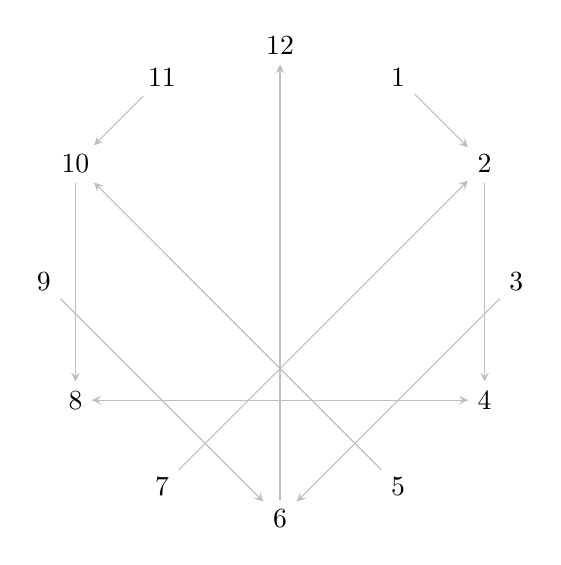
\begin{tikzpicture}
\node(A)at(0,3){12};\node(B)at(1.5,2.59807621){1};\node(C)at(2.59807621,1.5){2};\node(D)at(3,0){3};\node(E)at(2.59807621,-1.5){4};\node(F)at(1.5,-2.59807621){5};\node(G)at(0,-3){6};\node(H)at(-1.5,-2.59807621){7};\node(I)at(-2.59807621,-1.5){8};\node(J)at(-3,-0){9};\node(K)at(-2.59807621,1.5){10};\node(L)at(-1.5,2.59807621){11};\draw[thin,color=lightgray,-stealth](B)--(C);\draw[thin,color=lightgray,-stealth](C)--(E);\draw[thin,color=lightgray,-stealth](D)--(G);\draw[thin,color=lightgray,-stealth](E)--(I);\draw[thin,color=lightgray,-stealth](F)--(K);\draw[thin,color=lightgray,-stealth](G)--(A);\draw[thin,color=lightgray,-stealth](H)--(C);\draw[thin,color=lightgray,-stealth](I)--(E);\draw[thin,color=lightgray,-stealth](J)--(G);\draw[thin,color=lightgray,-stealth](K)--(I);\draw[thin,color=lightgray,-stealth](L)--(K);
\end{tikzpicture}
\end{figure}
Abbildung \ref{fig:2} stellt jede Multiplikation mit 2 durch einen Pfeil dar, wobei der Zahlenbereich auf 12 beschränkt ist. So entspricht \(2^3 \cdot 5\) Uhr natürlich nicht 40 Uhr, sondern 4 Uhr. Des Weiteren besteht hier die Möglichkeit, den Zahlenbereich beliebig zu erweitern.

\begin{figure}[ht]\centering
\caption{Zifferblätter erweitert auf 33 Ziffern}
\label{fig:3}
\vspace{6pt}
\hfill
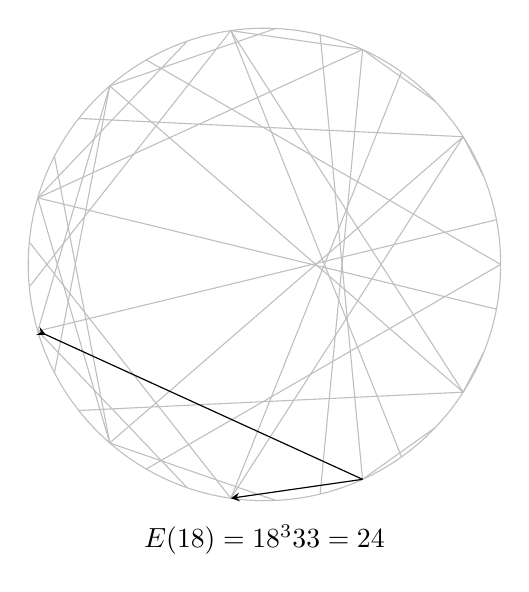
\begin{tikzpicture}
\draw[thin,color=lightgray](2.94578609,0.56775373)to(-2.87847892,-0.84519767);\draw[thin,color=lightgray](2.78510380,1.11498737)to(2.52376060,1.62192245);\draw[thin,color=lightgray](2.52376060,1.62192245)to(-1.96458220,-2.26724872);\draw[thin,color=lightgray](2.17120211,2.07023703)to(1.24624504,2.72889599);\draw[thin,color=lightgray](1.74017073,2.44372786)to(-0.42694451,-2.96946433);\draw[thin,color=lightgray](1.24624504,2.72889599)to(-0.42694451,2.96946433);\draw[thin,color=lightgray](0.70727681,2.91543470)to(1.24624504,-2.72889599);\draw[thin,color=lightgray](0.14274575,2.99660202)to(-1.96458220,2.26724872);\draw[thin,color=lightgray](-0.42694451,2.96946433)to(2.52376060,-1.62192245);\draw[thin,color=lightgray](-0.98120389,2.83500246)to(-2.87847892,0.84519767);\draw[thin,color=lightgray](-1.50000000,2.59807621)to(3.00000000,0.00000000);\draw[thin,color=lightgray](-1.96458220,2.26724872)to(-2.87847892,-0.84519767);\draw[thin,color=lightgray](-2.35815928,1.85447696)to(2.52376060,1.62192245);\draw[thin,color=lightgray](-2.66650635,1.37467957)to(-1.96458220,-2.26724872);\draw[thin,color=lightgray](-2.87847892,0.84519767)to(1.24624504,2.72889599);\draw[thin,color=lightgray](-2.98641577,0.28516813)to(-0.42694451,-2.96946433);\draw[thin,color=lightgray](-2.98641577,-0.28516813)to(-0.42694451,2.96946433);\draw[thin,color=lightgray](-2.87847892,-0.84519767)to(1.24624504,-2.72889599);\draw[thin,color=lightgray](-2.66650635,-1.37467957)to(-1.96458220,2.26724872);\draw[thin,color=lightgray](-2.35815928,-1.85447696)to(2.52376060,-1.62192245);\draw[thin,color=lightgray](-1.96458220,-2.26724872)to(-2.87847892,0.84519767);\draw[thin,color=lightgray](-1.50000000,-2.59807621)to(3.00000000,0.00000000);\draw[thin,color=lightgray](-0.98120389,-2.83500246)to(-2.87847892,-0.84519767);\draw[thin,color=lightgray](-0.42694451,-2.96946433)to(2.52376060,1.62192245);\draw[thin,color=lightgray](0.14274575,-2.99660202)to(-1.96458220,-2.26724872);\draw[thin,color=lightgray](0.70727681,-2.91543470)to(1.24624504,2.72889599);\draw[thin,color=lightgray](1.24624504,-2.72889599)to(-0.42694451,-2.96946433);\draw[thin,color=lightgray](1.74017073,-2.44372786)to(-0.42694451,2.96946433);\draw[thin,color=lightgray](2.17120211,-2.07023703)to(1.24624504,-2.72889599);\draw[thin,color=lightgray](2.52376060,-1.62192245)to(-1.96458220,2.26724872);\draw[thin,color=lightgray](2.78510380,-1.11498737)to(2.52376060,-1.62192245);\draw[thin,color=lightgray](2.94578609,-0.56775373)to(-2.87847892,0.84519767);\draw[thin,color=lightgray](3.00000000,-0.00000000)to(3.00000000,0.00000000);\draw[color=lightgray](0,0)circle( 3.000000000E+00);\draw[thin,stealth reversed-](-2.87847892,-0.84519767)to(1.24624504,-2.72889599);\draw[thin,-stealth](1.24624504,-2.72889599)to(-0.42694451,-2.96946433);\node(T)at(0,-3.5) {\(E(18) = 18^{3}\mod 33 = 24\)};
\end{tikzpicture}
\hfill
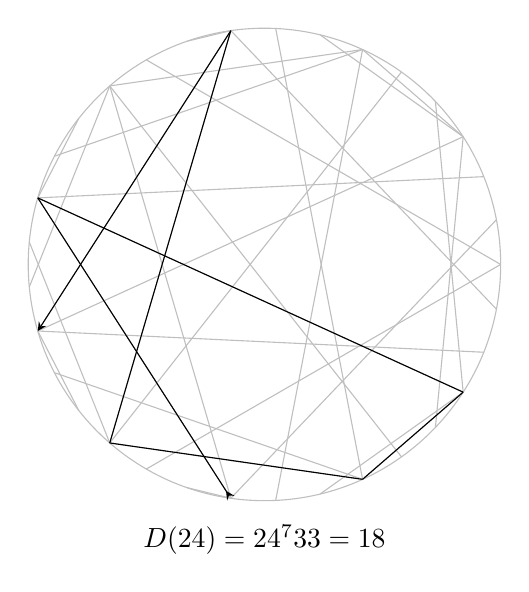
\begin{tikzpicture}
\draw[thin,color=lightgray](2.94578609,0.56775373)to(-0.42694451,-2.96946433);\draw[thin,color=lightgray](2.78510380,1.11498737)to(-2.87847892,0.84519767);\draw[thin,color=lightgray](2.52376060,1.62192245)to(1.24624504,2.72889599);\draw[thin,color=lightgray](2.17120211,2.07023703)to(2.52376060,-1.62192245);\draw[thin,color=lightgray](1.74017073,2.44372786)to(-1.96458220,-2.26724872);\draw[thin,color=lightgray](1.24624504,2.72889599)to(-1.96458220,2.26724872);\draw[thin,color=lightgray](0.70727681,2.91543470)to(2.52376060,1.62192245);\draw[thin,color=lightgray](0.14274575,2.99660202)to(1.24624504,-2.72889599);\draw[thin,color=lightgray](-0.42694451,2.96946433)to(-2.87847892,-0.84519767);\draw[thin,color=lightgray](-0.98120389,2.83500246)to(-0.42694451,2.96946433);\draw[thin,color=lightgray](-1.50000000,2.59807621)to(3.00000000,0.00000000);\draw[thin,color=lightgray](-1.96458220,2.26724872)to(-0.42694451,-2.96946433);\draw[thin,color=lightgray](-2.35815928,1.85447696)to(-2.87847892,0.84519767);\draw[thin,color=lightgray](-2.66650635,1.37467957)to(1.24624504,2.72889599);\draw[thin,color=lightgray](-2.87847892,0.84519767)to(2.52376060,-1.62192245);\draw[thin,color=lightgray](-2.98641577,0.28516813)to(-1.96458220,-2.26724872);\draw[thin,color=lightgray](-2.98641577,-0.28516813)to(-1.96458220,2.26724872);\draw[thin,color=lightgray](-2.87847892,-0.84519767)to(2.52376060,1.62192245);\draw[thin,color=lightgray](-2.66650635,-1.37467957)to(1.24624504,-2.72889599);\draw[thin,color=lightgray](-2.35815928,-1.85447696)to(-2.87847892,-0.84519767);\draw[thin,color=lightgray](-1.96458220,-2.26724872)to(-0.42694451,2.96946433);\draw[thin,color=lightgray](-1.50000000,-2.59807621)to(3.00000000,0.00000000);\draw[thin,color=lightgray](-0.98120389,-2.83500246)to(-0.42694451,-2.96946433);\draw[thin,color=lightgray](-0.42694451,-2.96946433)to(-2.87847892,0.84519767);\draw[thin,color=lightgray](0.14274575,-2.99660202)to(1.24624504,2.72889599);\draw[thin,color=lightgray](0.70727681,-2.91543470)to(2.52376060,-1.62192245);\draw[thin,color=lightgray](1.24624504,-2.72889599)to(-1.96458220,-2.26724872);\draw[thin,color=lightgray](1.74017073,-2.44372786)to(-1.96458220,2.26724872);\draw[thin,color=lightgray](2.17120211,-2.07023703)to(2.52376060,1.62192245);\draw[thin,color=lightgray](2.52376060,-1.62192245)to(1.24624504,-2.72889599);\draw[thin,color=lightgray](2.78510380,-1.11498737)to(-2.87847892,-0.84519767);\draw[thin,color=lightgray](2.94578609,-0.56775373)to(-0.42694451,2.96946433);\draw[thin,color=lightgray](3.00000000,-0.00000000)to(3.00000000,0.00000000);\draw[color=lightgray](0,0)circle( 3.000000000E+00);\draw[thin,stealth reversed-](-0.42694451,-2.96946433)to(-2.87847892,0.84519767);\draw[thin](-2.87847892,0.84519767)to(2.52376060,-1.62192245);\draw[thin](2.52376060,-1.62192245)to(1.24624504,-2.72889599);\draw[thin](1.24624504,-2.72889599)to(-1.96458220,-2.26724872);\draw[thin](-1.96458220,-2.26724872)to(-0.42694451,2.96946433);\draw[thin,-stealth](-0.42694451,2.96946433)to(-2.87847892,-0.84519767);\node(T)at(0,-3.5) {\(D(24) = 24^{7}\mod 33 = 18\)};
\end{tikzpicture}
\hfill
\end{figure}
Bezugnehmend auf das vorherige Beispiel ist links die Chiffrierung und rechts die Dechiffrierung dargestellt. Links repräsentiert jede graue Linie eine Multiplikation mit 18. Rechts ist dagegen eine Multiplikation mit 24 dargestellt. Der schwarze Pfad repräsentiert gerade den Sonderfall der modularen Exponentiation, also die Chiffrierung beziehungsweise Dechiffrierung.

\newpage

\pagenumbering{gobble}

\bibliographystyle{unsrt}
\bibliography{Rivest-Shamir-Adleman-Kryptosystem}

\end{document}
